\section{结合{GEM}的{LibContinual}模型}
\subsection{GEM~(LCL-8)项目简介}
\subsubsection{项目代码结构}
论文项目代码主要结构如下: 
\dirtree{%
    .1 \lstinline{LCL-8/}.
        .2 \lstinline{README.md}.
        .2 \lstinline{data/}.
            .3 \lstinline{cifar100.py}.
            .3 \lstinline{mnist_permutations.py}.
            .3 \lstinline{mnist_rotations.py}.
            .3 \lstinline{raw/}.
                .4 \lstinline{raw.py}.
        .2 \lstinline{main.py}.
        .2 \lstinline{metrics/}.
            .3 \lstinline{__init__.py}.
            .3 \lstinline{metrics.py}.
        .2 \lstinline{model/}.
            .3 \lstinline{__init__.py}.
            .3 \lstinline{common.py}.
            .3 \lstinline{ewc.py}.
            .3 \lstinline{gem.py}.
            .3 \lstinline{icarl.py}.
            .3 \lstinline{independent.py}.
            .3 \lstinline{multimodal.py}.
            .3 \lstinline{single.py}.
        .2 \lstinline{requirements.txt}.
        .2 \lstinline{results}.
            .3 \lstinline{plot_results.py}.
}

其中 \lstinline{model/gem.py} 为 GEM 算法的主要实现, \lstinline{data/}, \lstinline{metrics/} 分别是数据处理和结果评估部分. 我们接下来分别解析
\subsubsection{GEM算法内部函数解析}

\noindent\textbf{主体算法部分 \lstinline{Net} 类}
\begin{itemize}
    \item \lstinline{__init__}: 初始化GEM算法神经网络的结构和参数, 包括网络结构、损失函数、优化器、内存分配等
    \item \lstinline{forward(self, x, t)}: 前向迁移函数. 它确保只预测当前任务内的类别. 通过在输出张量的适当位置填充负无穷大值, 以确保不会选择超出当前任务范围的类别. 
    \item \lstinline{observe(self, x, t, y)}: 观察函数. 是GEM算法的核心, 通过更新内存和学习新示例处理灾难性遗忘问题. 在学习新任务时保存过去任务的梯度, 并在需要时进行投影, 模型可以更好地保留先前学到的知识. 
    具体分为以下步骤: 
    \begin{enumerate}
        \item 内存更新: 将来自当前任务的一批样本存储在内存中
        \item 先前任务的梯度计算: 遍历已观察到的任务列表, 对内存中存储的过去任务样本执行前向迁移和反向迁移, 计算梯度. 
        \item 当前任务的梯度计算: 对当前任务的小批量样本执行前向迁移和反向迁移, 计算梯度. 
        \item 梯度约束检查: 如果已经观察了多个任务, 检查当前任务的梯度是否违反了约束. 如果违反, 使用GEM投影进行修正. 
        \item 应用梯度: 将梯度应用于模型参数, 并进行优化. 
    \end{enumerate}
    
\end{itemize}

\noindent\textbf{剩余辅助函数}
\begin{itemize}
    \item \lstinline{compute_offsets(task, nc_per_task, is_cifar)}: 算用于数据集的偏移, 确定为给定任务选择哪些输出. 
    \item \lstinline{store_grad(pp, grads, grad_dims, tid)}: 存储过去任务的参数梯度. 
    \item \lstinline{overwrite_grad(pp, newgrad, grad_dims)}: 用新的梯度向量覆盖梯度, 以纠正违规. 
    \item \lstinline{project2cone2(gradient, memories, margin=0.5, eps=1e-3)}: 解决GEM论文中描述的二次规划问题, 用于给定提议的梯度和任务梯度内存, 覆盖梯度以进行最终投影更新. 
\end{itemize}
        

\subsection{LibContinual项目简介}
\subsubsection{LibContinual框架架构} 
通过阅读框架源码, 该LibContinual持续学习框架将持续学习的步骤抽象, 分出5大模块: 
\begin{enumerate}
    \item \textit{config模块}: 位于 \lstinline{config/}, 负责\textbf{整个训练过程的参数配置}. 新增算法时, 为每个方法在该路径下新建一个yaml文件, 再在 \lstinline{run_trainer.py} 里填入各自方法对应的yaml配置文件路径.  
    \item \textit{data模块}: 位于 \lstinline{core/data}, 负责\textbf{数据集的读取}. dataloader.py负责根据配置信息初始化数据加载器,  dataset.py负责创建和管理连续学习任务的数据集. 可以在dataloader.py添加预处理(transform)的逻辑. 
    \item \textit{model模块}: 位于 \lstinline{core/model}, 负责\textbf{机器学习模型的定义}, 包括backbone模型骨架、buffer模型缓存、replay模型传播算法三个部分. 
    \item \textit{trainer模块}: 位于 \lstinline{core/trainer.py}, 负责\textbf{整个实验的流程控制}. 
        \begin{enumerate}
        \item 通过util类中的 \lstinline{get_instance ()} 方法, 获取其他模块的对象. 
        \item 目前抽象得不够完善, 新增部分算法时需要修改 \lstinline{train_loop}函数以实现部分功能. 
        \end{enumerate}
    \item \textit{utils模块}: \lstinline{core/utils/} 训练过程中用到的\textbf{工具类}. 目前包含Logger日志输出类、AverageMeter指标计算类、字符串格式化方法等工具. 
\end{enumerate}
\begin{figure}[H]
    \centering
    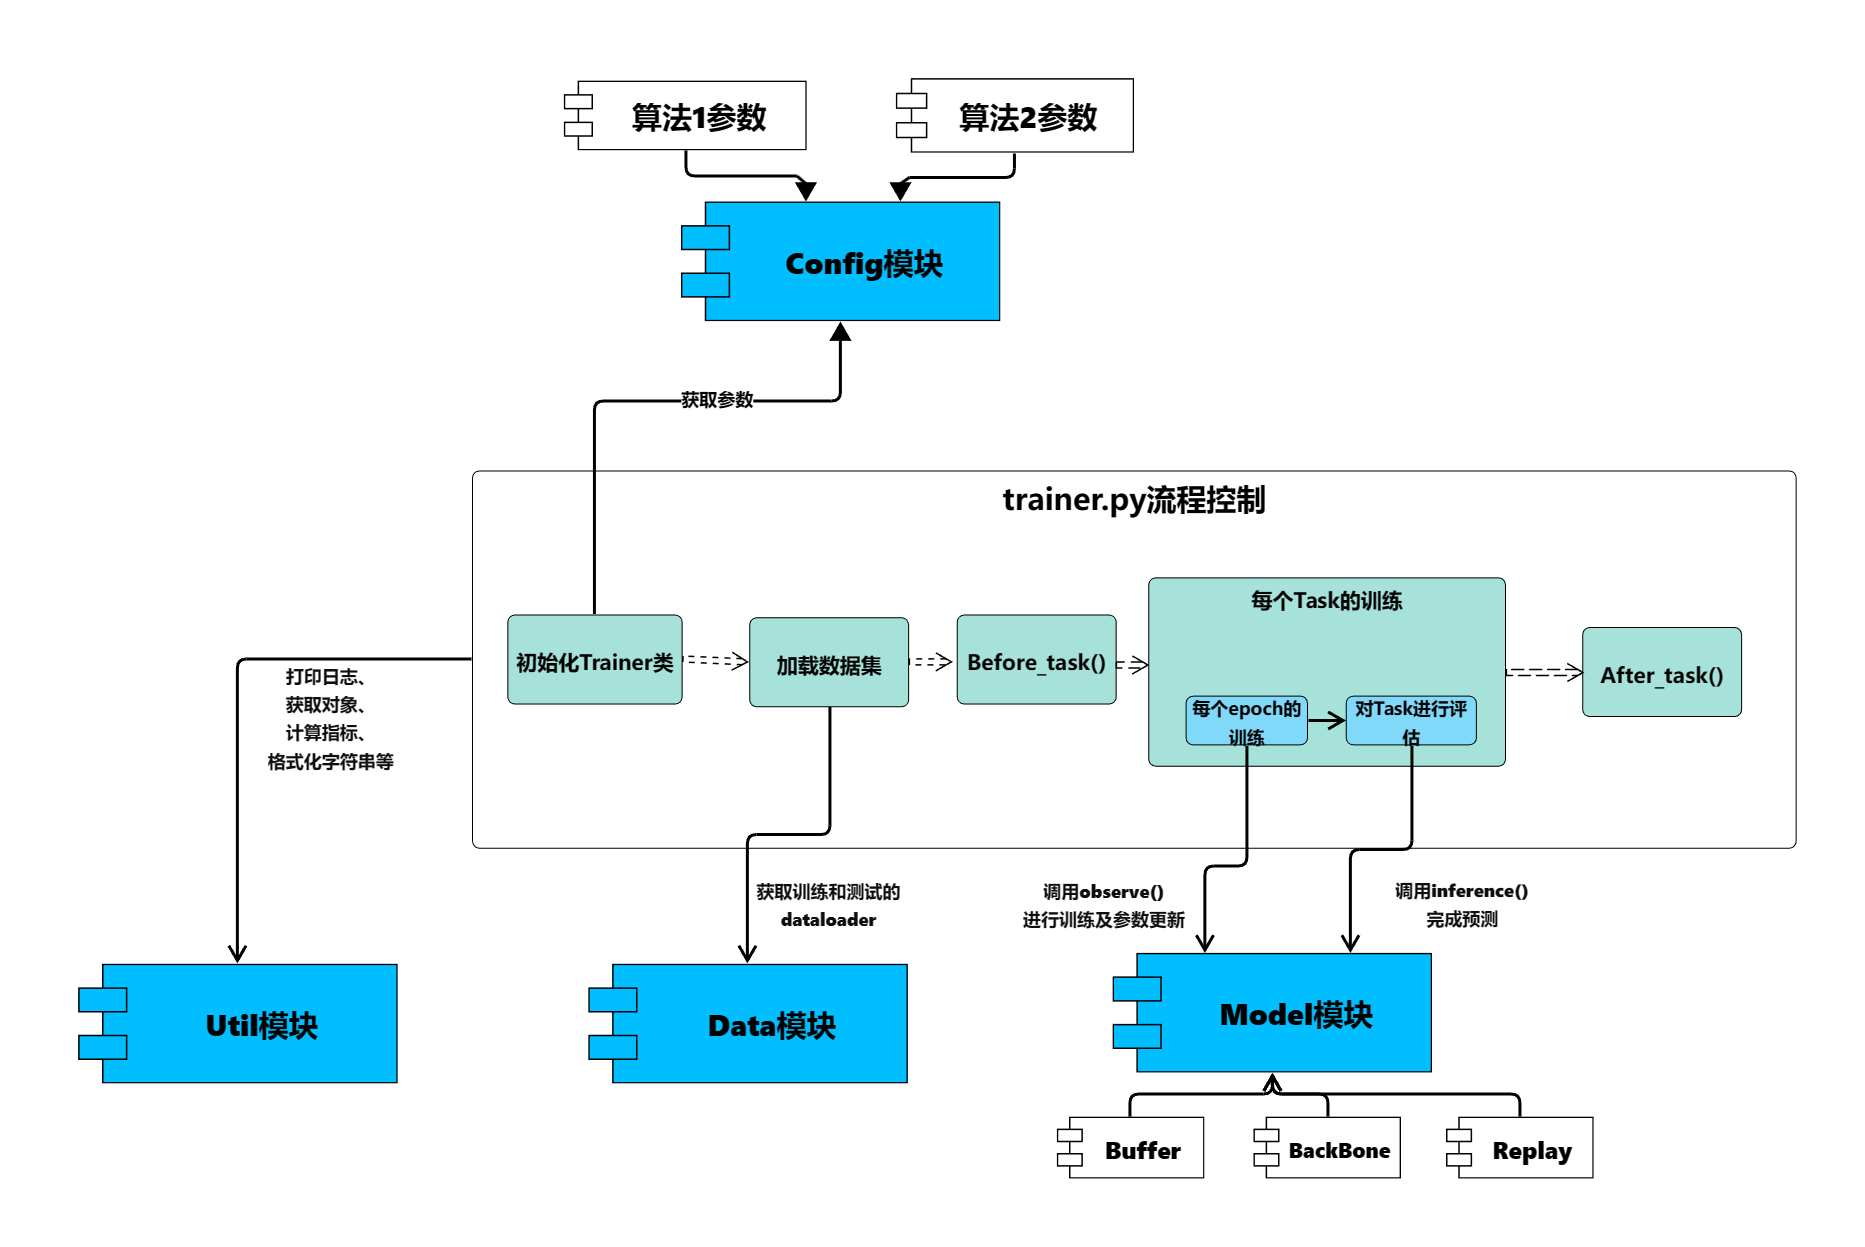
\includegraphics[width=1\linewidth]{modules.png}
    \caption{模块依赖图}
    \label{fig:框架图}
\end{figure}

\subsubsection{训练流程解析}

\textbf{入口函数}: 框架入口为根目录下的\lstinline{run_trainer.py}. 修改 \lstinline{config} 中的配置类即可选择运行测试哪一个持续学习框架. 

\textbf{构建 \lstinline{class Train}}:进入 \lstinline{main()} 函数, 首先记录当前时间, 随后从配置类构建 \lstinline{class Train}. 依次初始化必要信息: 日志记录器 \lstinline{logger}, 设备 \lstinline{device} (目前不支持分布式多gpu训练) 、总任务数 \lstinline{task_num}, 模型 \lstinline{model}, 缓冲区 \lstinline{buffer}, 优化器 \lstinline{optimizer}, 学习率调度器 \lstinline{scheduler}, 计量器 \lstinline{train_meter} 和 \lstinline{test_meter} 等. 

\textbf{每个Task的训练循环}: 初始化完成后, 进入主循环 \lstinline{train_loop()}, \textbf{负责每一轮task的流程控制}. 
\begin{enumerate}
    \item 在每个task开始前, 会执行 \lstinline{before_task()} 方法, 初始化优化器和学习率调度器, 并调整缓冲区的总类别数.  (如果缓冲区的策略是线性缓冲区 (LinearBuffer) , 会将缓冲区的图像和标签添加到数据集中, 并重新创建数据加载器) 
    \item 进入每个训练周期epoch的循环后, 会调用\lstinline{_train()}函数进行训练, 并打印损失和平均准确率. 如果达到了验证周期 (\lstinline{val_per_epoch}) 或者是最后一个训练周期, 会调用\lstinline{_validate()}函数进行测试, 并更新最佳准确率. 随后更新学习率. 
    \begin{itemize}
    \item \lstinline{_train()}函数: 位于 \lstinline{core/trainer.py} , \textbf{负责每一轮epochs的模型训练}. 它接受两个参数: \lstinline{epoch_idx} 表示当前的训练轮数, dataloader是一个数据加载器, 用于加载训练数据. 
    函数内部初始化一个计量器meter用于记录训练过程中的指标. 接下来通过一个循环遍历dataloader中的每个batch数据. 对于每个batch, 模型会根据输入数据进行前向传播, 计算输出、准确率和损失. 然后使用优化器将损失反向传播并更新模型的参数. 最后, 计量器meter更新准确率指标. 
    \item \lstinline{_validate()}函数: 位于 \lstinline{core/trainer.py}, \textbf{负责验证当前模型在之前所有任务上的性能}, 防止遗忘. 它接受一个参数 \lstinline{task_idx}, 表示当前的任务索引. 
    函数内部首先根据任务索引获取相应的数据加载器dataloader. 然后初始化一个计量器meter用于记录验证过程中的指标. 接下来通过一个循环遍历dataloader中的每个batch数据. 对于每个batch, 模型会根据输入数据进行推断, 计算输出和准确率. 然后计量器更新准确率指标. 最后将每个任务的平均准确率和每个任务的准确率列表返回. 
\end{itemize}
    \item 在每个任务结束之后, 会执行 \lstinline{after_task()} 方法, 并根据缓冲区的策略进行缓冲区的更新操作. 
\end{enumerate}

\textbf{循环出口: }结束所有Task的训练与测试. 

\subsubsection{框架核心部分解析: }即新增持续学习算法的核心函数, 扩展性较强, 包括构成 \lstinline{model} 的几个模块. 
\begin{itemize}
\item \textit{replay模块}: 位于 \lstinline{core/model/replay}, 负责 \textbf{具体持续学习算法的定义}. 
    \begin{enumerate}
    \item \lstinline{def __init__()}:  用来初始化各自算法需要的对象
    \item \lstinline{def observe(self, data)}:  \textbf{训练}过程中, 面对到来的一个batch的样本完成训练的损失计算以及参数更新, 返回 \lstinline{pred}, \lstinline{acc}, \lstinline{loss} (预测结果, 准确率, 损失)
    \item \lstinline{def inference(self, data)}: \textbf{推理}过程中, 面对到来的一个batch的样本, 完成预测, 返回 \lstinline{pred}, \lstinline{acc}
    \item \lstinline{def before_task() / def after_task()}: 如果算法在每个任务开始前后有额外的操作, 在这两个函数内完成 
    \end{enumerate}
\item \textit{bakcbone模块}: 位于 \lstinline{core/model/backbone}, 负责\textbf{backbone模型文件的定义}. 
    \begin{enumerate}
    \item 定义卷积层, 池化层和激活函数, 不负责定义全连接层. 
    \item 目前只有 \lstinline{resnet.py} 文件中包含了 \lstinline{resnet18}, \lstinline{resnet34}, \lstinline{resnet50} 等模型骨架, 可以添加其他 \lstinline{model} 的 \lstinline{backbone.py}, 以适配不同的持续学习算法
    \end{enumerate}
\item \textit{buffer模块}: 位于 \lstinline{core/model/buffer}, 负责
\textbf{训练过程中buffer的管理以及更新}. 
    \begin{enumerate}
        \item 新增文件以添加Buffer类型: 目前实现了 \lstinline{LinearBuffer} 和 \lstinline{HerdingBuffer}, 在每个任务开始前会把buffer样本与新样本拼接在一起. 
        \item 更新策略: 在 \lstinline{update.py}. 目前支持random更新和hearding更新.  
    \end{enumerate}
\end{itemize}



\subsection{将GEM模型集成到LibContinual中}
为了将GEM模型加入到LibContinual库中, 我们主要进行了如下的修改. 
\subsubsection{\texorpdfstring{添加 \lstinline{gem.py}}{添加 gem.py}}

\lstinline{gem.py} 模型主要的控制部分, 用于控制GEM算法的训练和推理过程. 值得注意的是, GEM原本的代码将所有的数据放在一起训练, 并未分成不同的任务. 具体表现在原本的循环写法是这样的:
\begin{lstlisting}[language=python]
    for (i, (x, task_idx, y)) in enumerate(tqdm(dataloader)):
\end{lstlisting}
而在LibContinual中, 我们的训练过程是按照任务进行的, 明显表现在循环写法上是这样的:
\begin{lstlisting}[language=python]
    for task_idx in range(self.task_num):
        for epoch_idx in range(self.init_epochs):
\end{lstlisting}

总的来说, 原文中GEM模型对应的 \lstinline{class GEM} 具有更多的职责. 在类的外部调用时, 只需要加以简单的刻画, 就可以完成训练和测试. 但是 \lstinline{LibContinual} 中所有的模型类都被赋予了更有限的职责, 因此我们的主要工作就是对GEM的代码解耦合, 将大量的职责分开, 嵌入到给定的库代码的对应部分.


\subsubsection{\texorpdfstring{修改 \lstinline{trainer.py}}{修改 trainer.py}}
和上述 \lstinline{gem.py} 对应的, \lstinline{trainer.py} 中的修改的部分也基本是相应的解耦合. 原本的GEM代码更像是结构式编程, 而 \lstinline{LibContinual} 中的代码更像是面向对象编程. 因此, 我们将原本的代码中的对应功能修改为了类的对应的成员变量和成员函数. 具体可以查看代码.

\subsubsection{其余修改}
为了实现上述的两大点修改, 我们还进行了大量的修改, 包括但不限于:
\begin{itemize}
    \item 添加\lstinline{ringbuffer.py}作为单独的buffer对象.
    \item 添加\lstinline{metics.py}用作评价指标.
    \item 大量修改\lstinline{dataloader.py}和\lstinline{dataset.py}中的代码, 以适配GEM模型的训练和测试. 
    \item 由于GEM模型使用的是二进制 \lstinline{cifar100} 数据集, 因此我们大量修改了数据的读取, 处理和预处理部分的代码.
\end{itemize}

\subsubsection{一些尝试}
为了从软件工程的角度将GEM的代码更好地融入到LibContinual中, 我们还尝试了一些其他的方法, 但是由于时间和能力的限制, 并没有成功. 以下是我们进行的尝试.
\begin{itemize}
    \item \lstinline{cifar100}有几种不同格式的数据集, LibContinual使用的是image格式, 而GEM使用的是binary格式的数据集, 我们试着将binary数据的处理和image数据的处理结合起来, 使得一种方法可以同时处理两种数据, 但是我们并未成功.
    \item 现在论文中有不少 \lstinline{if-else} 的写法, 因为GEM与LibContinual的差距实在太大, 我们难以将所有的 \lstinline{if-else} 都去掉. 我们尝试利用面向对象函数的重载, 来减少控制流的使用. 由于Python中并不支持传统的函数重载, 因此我们充分利用函数参数的默认值, 尽我们的能力减少了 \lstinline{if-else} 的使用, 但是由于时间和能力的限制, 仍然保留了一部分.
    \item 我们试着将 \lstinline{class GEM} 的职责完全抽离开来, 使得 \lstinline{task_idx} 不作为参数传入. 这需要改动大量的代码, 几乎是重写了 \lstinline{class GEM} 的所有代码. 我们只在一定程度上实现了这一点, 虽然在效果上和原来的模型几乎无差距, 但是从软件工程项目架构的角度来看, 这一部分仍然需要改进.
\end{itemize}
